\documentclass[11pt,spanish,a4paper]{article}
\usepackage[utf8]{inputenc}
\usepackage[spanish,es-nodecimaldot]{babel}
\usepackage{times}
\usepackage{graphicx}
\usepackage{amsmath,amssymb}
\usepackage{multicol}
\oddsidemargin=0.5cm
\textwidth=15cm
\textheight=50\baselineskip
\topmargin=-1.5cm
\parskip 1em
%\parindent 0pt

\begin{document}
%\renewcommand{\labelenumi}{\em \alph{enumi})}
%\renewcommand{\labelenumii}{\em \arabic{enumii})}
\newcommand\al{\alpha}
\newcommand\noi{\noindent}
\newcommand\re{\mbox{Re}}
\newcommand\im{\mbox{Im}}
%\newcommand\arg{\mbox{arg}}
\newcommand\Arg{\mbox{Arg}}

\title{Escribiendo en latex}

\author{Matias Valle}

\maketitle

\section{Matematicas}

\subsection{Expresiones Matematicas}
\begin{enumerate}

\item $a^2 + b^2 = c^2$

\item $ \displaystyle x_{1,2} = \frac{-b\pm \sqrt{b^2-4ac}}{2a} $

\item $a = \frac{1}{b+\frac{1}{c+\frac{1}{d+\cdots}}}$

\item $f(x) = \sqrt[3]{\frac{x^2-2x+3}{x-1}}$

\item $\frac{\sin(\alpha)}{\cos(\alpha)} \neq \frac{\cos(-\alpha)}{\sin(-\alpha)} $

\item $\displaystyle \int_0^\infty \sin(t) e^{-t^2} dt < \infty $

\item $ \displaystyle \sum_{n=0}^{\infty} a_n = \lim\limits_{N\to\infty} \sum_{n=0}^{N} a_n$ 

\end{enumerate}

\subsection{Teoremas}
\begin{itemize}
\item {\bfseries\itshape Segundo Teorema Fundamental del Calculo:} Sea $f(x)$ una funcion continuaen el intervalo [a,b] y F(x) cualquier funcion primitiva de f, es decir, tal qie $F'(x)=f(x) \forall x \epsilon [a,b]$. luego

\[\int_a^b f(x) dx = F(b)-F(a)\]

\item {\bfseries\itshape Pequeno teorema de Fermat:} Si p es un numero primo y a $\epsilon$ N, se tiene que $a^p \equiv a$ modulo p 
\end{itemize}

%%%%%%%%%%%%%%%%%%%%%%%%%%%%%%%%%%%%%%%%%%%%%%%%%%%%%
\break
\subsection{Problema 2}

%\begin{figure}
%\centering
%\includegraphics[width = 0.6\textwidth]{daleque.png}
%\caption{\label{fig:daleque}Grafico de $f(x)= e^x sin(x)$}
%\end{figure}

\begin{figure}[h]
\begin{center}
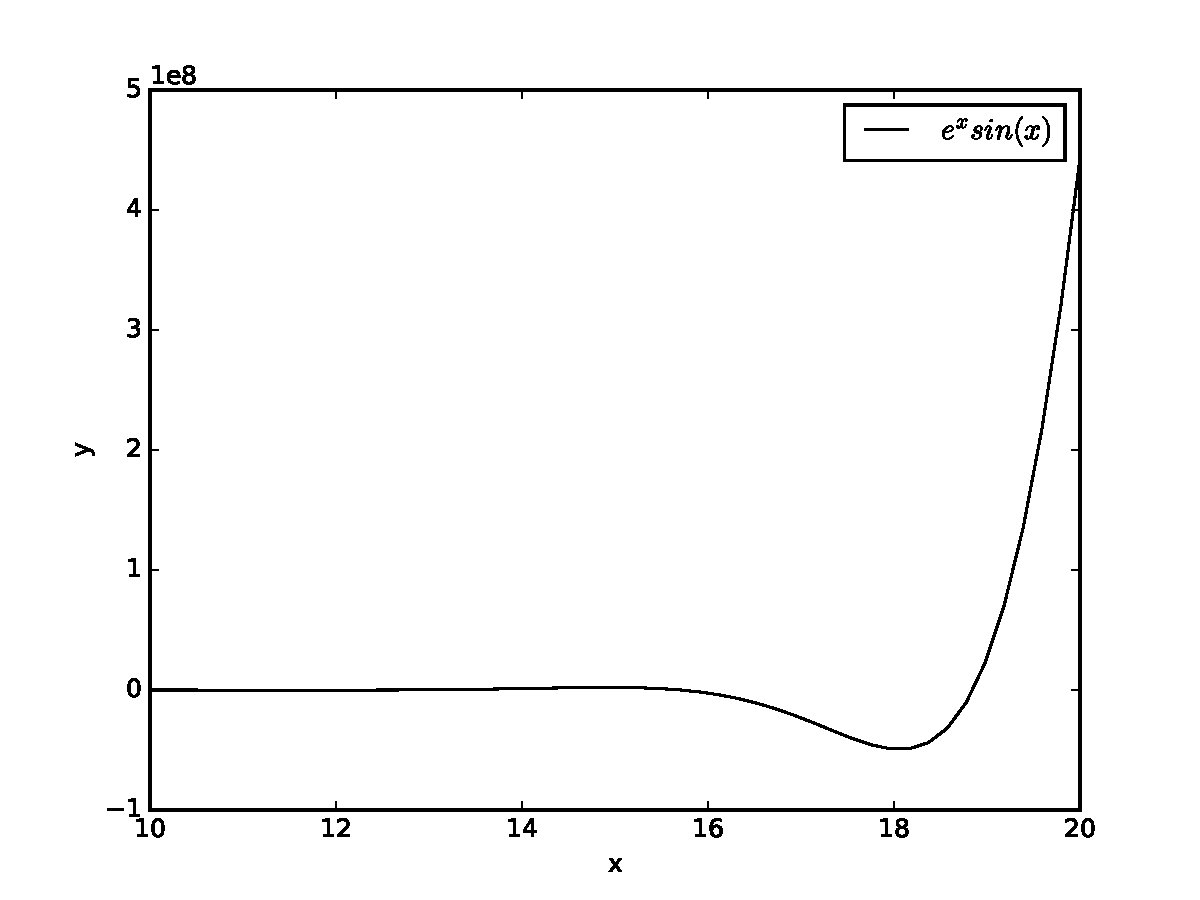
\includegraphics[width=9cm]{graf.pdf}
\caption{Grafico de $f(x)= e^x sin(x)$ }\label{plot1}
\end{center}
\end{figure}

%%%%%%%%%%%%%%%%%%%%%%%%%%%%%%%%%%%%%%%%%%%%%%%%%%%%%%

\subsection{Problema 3}


\begin{table}[h]
\begin{tabular}{l|r}
$x$ & $f(x)$\\\hline\hline
2 & 1/2 \\
1 & 1/2 \\
1/2 & 4/5 \\
0 & 1 \\
-1 & 1/2 \\
-2 & 1/5 \\ \hline
\end{tabular}
\end{table}

\begin{minipage}{0.4\hsize}
%\begin{figure}
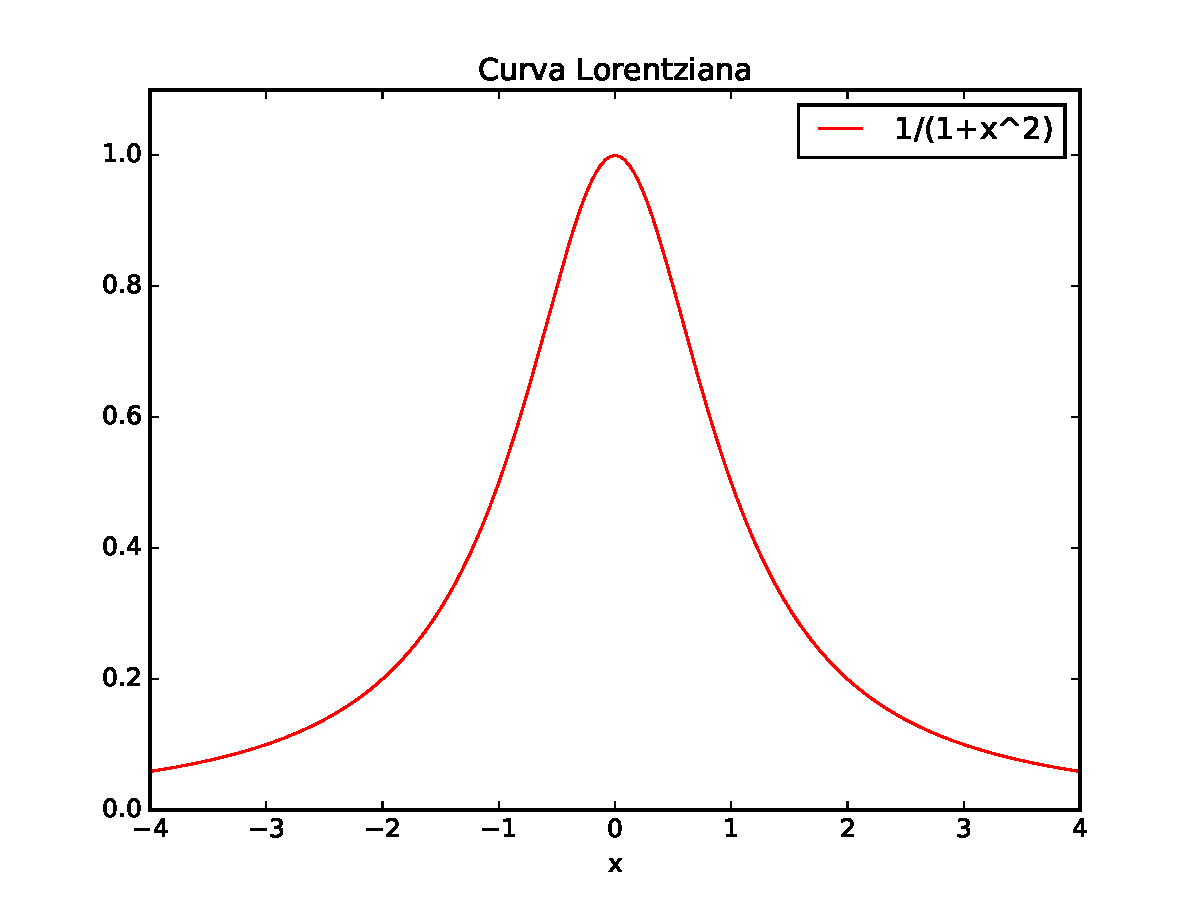
\includegraphics[width=5.5cm]{lorentziana.pdf}
\end{minipage}
%\caption{Grafico de la funcion Lorentziana}\label{plot1}
%\end{figure}

%%%%%%%%%%%%%%%%%%%%%%%%%%%%%%%%%%%%%%%%%%%%%%%%%%%%%%%%%%%%%%%%%%
\subsection{Problema 4}

\begin{table}[ht]
\centering
\begin{tabular}{|l||r|r|r|r|r|}\hline
 & {\bfseries\itshape Lunes} & {\bfseries\itshape Martes} & {\bfseries\itshape Miercoles} & {\bfseries\itshape Jueves} & {\bfseries\itshape Viernes}\\ \hline\hline
{\bfseries\itshape 8} & Matematica & Matematica & Musica & plastica & cs. naturales\\
{\bfseries\itshape 9} & matematica & matematica & cs.sociales & educ. fisica & cs.naturales\\
{\bfseries\itshape 10} & cs. naturales & lengua & cs. sociales & lengua & ingles \\
{\bfseries\itshape 11} & cs. naturales & lengua & cs. sociales & lengua & cs. sociales\\ \hline
\end{tabular}
\end{table}

%%%%%%%%%%%%%%%%%%%%%%%%%%%%%%%%%%%%%%%%%%%%%%%%%%%%%%%%%%%%%%%%%%%%%%%%
\subsection{Problema 5}

\begin{eqnarray*}
(a+b)^3 & = &  (a+b)(a+b)^2\\
& = & (a+b)(a^2+2ab+b^2)\\
& = & a^3+2a^2b+ab^2+ba^2+2ab^2+b^3\\
\end{eqnarray*}




\end{document}
